\documentclass[aspectratio=169]{beamer}

% =================================================================
%  Introduction to Robotics
%  A beginner-friendly Beamer deck (fully self-contained: all
%  figures / flowcharts / plots drawn with TikZ, so it compiles anywhere).
% =================================================================

% -------------------------------------------------
% Theme and packages
% -------------------------------------------------
\usetheme{Madrid}
\usecolortheme{default}

\usepackage{amsmath}
\usepackage{amssymb}
\usepackage{bm}
\usepackage{listings}
\usepackage{tikz}
\usepackage{array}
\usepackage{booktabs}
\usepackage{tabularx}
\usepackage{ragged2e}
\usepackage{xcolor}

\usetikzlibrary{shapes.geometric, arrows.meta, positioning, calc, fit, backgrounds, patterns}

% -------------------------------------------------
% Colour palette
% -------------------------------------------------
\definecolor{cAccent}{RGB}{0,102,153}     % teal-blue accent
\definecolor{cBox}{RGB}{28,31,42}          % dark box
\definecolor{cGreen}{RGB}{34,139,34}
\definecolor{cRed}{RGB}{178,34,34}
\definecolor{cOrange}{RGB}{204,102,0}
\definecolor{cPurple}{RGB}{102,45,145}
\definecolor{cGrayBg}{RGB}{245,246,248}
\definecolor{codebg}{RGB}{248,248,244}
\definecolor{codekw}{RGB}{0,0,180}
\definecolor{codecomment}{RGB}{0,130,0}
\definecolor{codestr}{RGB}{170,55,20}

% Beamer colour tweaks (match a Madrid-style accent)
\setbeamercolor{structure}{fg=cAccent}
\setbeamertemplate{frametitle continuation}{%
	\ifnum\insertcontinuationcount>1\space(cont...)\fi
}
\setbeamertemplate{navigation symbols}{}
\setbeamertemplate{caption}[numbered]

% -------------------------------------------------
% Listings style for C code
% -------------------------------------------------
\lstdefinestyle{cstyle}{
	language=C,
	backgroundcolor=\color{codebg},
	basicstyle=\ttfamily\footnotesize,
	keywordstyle=\color{codekw}\bfseries,
	commentstyle=\color{codecomment}\itshape,
	stringstyle=\color{codestr},
	numbers=none,
	numberstyle=\tiny\color{gray},
	numbersep=8pt,
	showstringspaces=false,
	breaklines=true,
	frame=single,
	rulecolor=\color{gray!50},
	tabsize=2,
	columns=fullflexible,
	keepspaces=true,
	literate={~}{{$\sim$}}1
}
\lstset{style=cstyle}

% Listings style for a robot language (VAL-like)
\lstdefinelanguage{val}{
	morekeywords={PROGRAM,APPRO,APPROS,MOVE,MOVES,DEPART,DEPARTS,OPENI,CLOSEI,SPEED,
		SIGNAL,WAITI,WAIT,END,HERE,SET},
	morecomment=[l]{;},
	sensitive=true
}
\lstdefinestyle{valstyle}{
	style=cstyle,
	language=val,
	breaklines=false,
	keywordstyle=\color{codekw}\bfseries,
	commentstyle=\color{codecomment}\itshape
}

% Handy TikZ flowchart node styles
\tikzset{
	startstop/.style={rectangle, rounded corners=10pt, minimum width=2.4cm, minimum height=0.8cm, text centered, align=center, draw=black, fill=cAccent!25},
	process/.style  ={rectangle, minimum width=2.6cm, minimum height=0.8cm, text centered, align=center, text width=2.8cm, draw=black, fill=blue!8},
	io/.style       ={trapezium, trapezium left angle=70, trapezium right angle=110, minimum width=2.2cm, minimum height=0.8cm, text centered, align=center, draw=black, fill=cOrange!20},
	decision/.style ={diamond, aspect=2, minimum width=2.4cm, minimum height=0.9cm, text centered, text width=2.2cm, draw=black, fill=cGreen!18, inner sep=1pt},
	flowarrow/.style={-{Stealth[length=2.5mm]}, thick},
	% block diagram styles
	blk/.style      ={rectangle, draw=black, thick, minimum width=1.9cm, minimum height=0.9cm, align=center, fill=blue!8},
	sumj/.style     ={circle, draw=black, thick, minimum size=0.55cm, inner sep=0pt},
	sig/.style      ={-{Stealth[length=2.2mm]}, thick},
	% robot drawing styles
	link/.style     ={line width=4pt, cOrange, line cap=round},
	joint/.style    ={circle, draw=black, thick, fill=white, minimum size=0.28cm, inner sep=0pt},
	ground/.style   ={pattern=north east lines, draw=none},
}

\setbeamertemplate{footnote}{%
	\parindent 0em
	\noindent
	\raggedright
	\insertfootnotemark\insertfootnotetext\par
}

% -------------------------------------------------
% Title information
% -------------------------------------------------
\title[Introduction to Robotics]{Introduction to Robotics}
\subtitle{Anatomy, Drives, End-Effectors, Controllers, Sensors \& Economics}
\author[Amit Kumar Singh]{}
\institute[]{
	Amit Kumar Singh \\
	\vspace{0.1cm}
	Assistant Professor (ECE) \\
	\vspace{0.05cm}
	School of Naval Architecture and Ocean Engineering\\
	\vspace{0.05cm}
	Indian Maritime University Visakhapatnam Campus, Sabbavaram Mandal\\
	\vspace{0.05cm}
	Visakhapatnam, Andhra Pradesh -- 531~035\\
	\vspace{0.25cm}
	amitkumarsingh@imu.ac.in
}
\date[AI \& Automation]{\today}

\begin{document}

	%------------------------------------------------
	\begin{frame}
		\titlepage
	\end{frame}

	%------------------------------------------------
	\begin{frame}{Outline}
		\small
		\begin{columns}[T,onlytextwidth]
			\hspace{0.8cm}% shift the first column to the right
			\begin{column}{0.49\textwidth}
				\tableofcontents[hideallsubsections, sections={1-5}]
			\end{column}
			\hspace{0.8cm}% wider gap between the two columns
			\begin{column}{0.40\textwidth}
				\tableofcontents[hideallsubsections, sections={6-9}]
			\end{column}
		\end{columns}
	\end{frame}

	% =================================================================
	\section{Introduction to Robotics}
	% =================================================================
	\begin{frame}{What is a Robot?}
		\begin{block}{Definition (Robot Institute of America)}
			An \textbf{industrial robot} is a \textbf{reprogrammable, multifunctional manipulator} designed to move
			material, parts, tools or special devices through \textbf{variable programmed motions} for the performance
			of a variety of tasks.
		\end{block}
		\vspace{0.2cm}
		\begin{columns}
			\begin{column}{0.58\textwidth}
				\begin{itemize}
					\item \textbf{Reprogrammable} --- a new task needs only a new program.
					\item \textbf{Multifunctional} --- the same arm can weld, paint, load or assemble.
					\item \textbf{Manipulator} --- an arm of links and joints that moves in space.
					\item A robot is the ``general-purpose NC machine'': it follows the same
					\textbf{sense $\rightarrow$ decide $\rightarrow$ act} cycle.
				\end{itemize}
			\end{column}
			\begin{column}{0.42\textwidth}
				\centering
				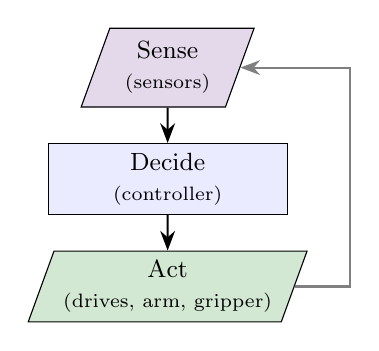
\begin{tikzpicture}[node distance=0.45cm, every node/.style={font=\small}]
					\node[io, fill=cPurple!18] (s) {Sense\\ \scriptsize(sensors)};
					\node[process, below=of s] (d) {Decide\\ \scriptsize(controller)};
					\node[io, below=of d, fill=cGreen!20] (a) {Act\\ \scriptsize(drives, arm, gripper)};
					\draw[flowarrow] (s) -- (d);
					\draw[flowarrow] (d) -- (a);
					\draw[flowarrow, gray] (a.east) -- ++(0.7,0) |- (s.east);
				\end{tikzpicture}
			\end{column}
		\end{columns}
	\end{frame}

	\begin{frame}{A Short History of Robotics}
		\centering
		\resizebox{\textwidth}{!}{%
			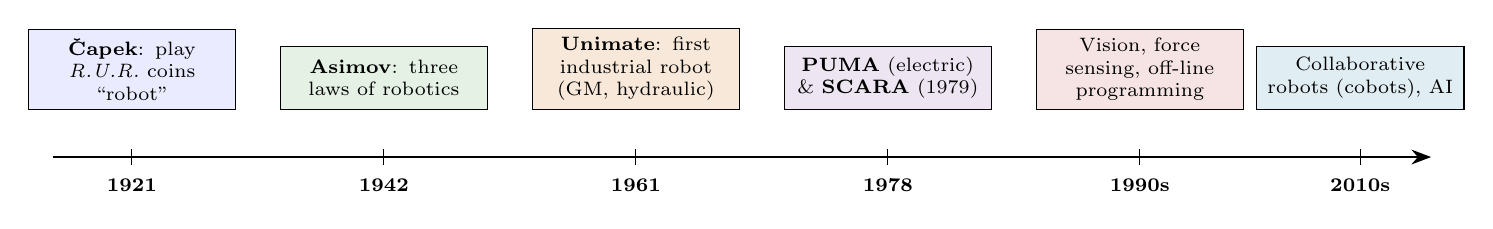
\begin{tikzpicture}[every node/.style={font=\scriptsize}]
				\draw[flowarrow, thick] (0,0) -- (17.5,0);
				\foreach \x/\yr in {1/1921, 4.2/1942, 7.4/1961, 10.6/1978, 13.8/1990s, 16.6/2010s} {
					\draw (\x,0.1) -- (\x,-0.1);
					\node[below] at (\x,-0.15) {\textbf{\yr}};
				}
				\node[process, fill=blue!8,    text width=2.4cm, above=0.6cm] at (1,0)    {\textbf{\v{C}apek}: play \emph{R.U.R.} coins ``robot''};
				\node[process, fill=cGreen!12, text width=2.4cm, above=0.6cm] at (4.2,0)  {\textbf{Asimov}: three laws of robotics};
				\node[process, fill=cOrange!15,text width=2.4cm, above=0.6cm] at (7.4,0)  {\textbf{Unimate}: first industrial robot (GM, hydraulic)};
				\node[process, fill=cPurple!12,text width=2.4cm, above=0.6cm] at (10.6,0) {\textbf{PUMA} (electric) \& \textbf{SCARA} (1979)};
				\node[process, fill=cRed!12,   text width=2.4cm, above=0.6cm] at (13.8,0) {Vision, force sensing, off-line programming};
				\node[process, fill=cAccent!12,text width=2.4cm, above=0.6cm] at (16.6,0) {Collaborative robots (cobots), AI};
		\end{tikzpicture}}
		\vspace{0.4cm}
		\begin{block}{Asimov's three laws (1942)}
			\small A robot may not injure a human; it must obey orders unless that breaks the first law; it must protect itself unless that breaks the first two laws.
		\end{block}
	\end{frame}

	\begin{frame}{Components of an Industrial Robot System}
		\centering
		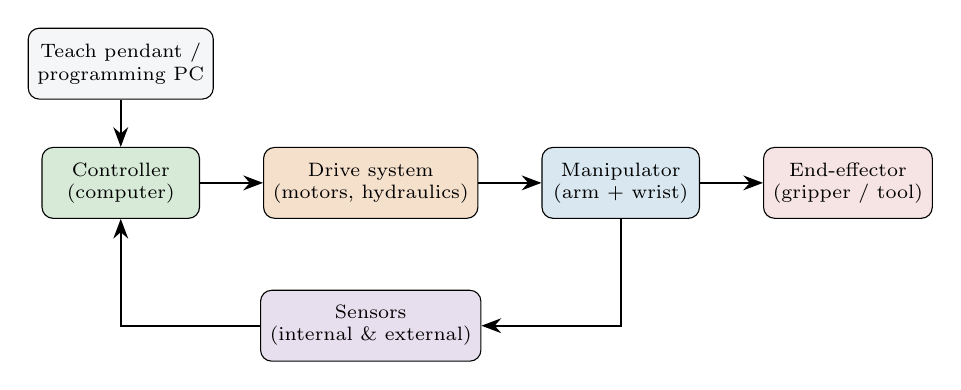
\begin{tikzpicture}[every node/.style={font=\scriptsize},
			el/.style={rectangle, draw=black, rounded corners, minimum width=2.0cm, minimum height=0.9cm, align=center, fill=blue!8}]
			\node[el, fill=cGreen!18] (ctrl) {Controller\\ (computer)};
			\node[el, right=0.8cm of ctrl, fill=cOrange!20] (drv) {Drive system\\ (motors, hydraulics)};
			\node[el, right=0.8cm of drv, fill=cAccent!15] (man) {Manipulator\\ (arm + wrist)};
			\node[el, right=0.8cm of man, fill=cRed!12] (ee) {End-effector\\ (gripper / tool)};
			\node[el, below=0.9cm of drv, fill=cPurple!15] (sen) {Sensors\\ (internal \& external)};
			\node[el, above=0.6cm of ctrl, fill=cGrayBg] (tp) {Teach pendant /\\ programming PC};
			\draw[flowarrow] (tp) -- (ctrl);
			\draw[flowarrow] (ctrl) -- (drv);
			\draw[flowarrow] (drv) -- (man);
			\draw[flowarrow] (man) -- (ee);
			\draw[flowarrow] (man.south) |- (sen.east);
			\draw[flowarrow] (sen.west) -| (ctrl.south);
		\end{tikzpicture}
		\vspace{0.25cm}
		\begin{itemize}\small
			\item \textbf{Manipulator} --- the mechanical arm: base, links, joints and wrist.
			\item \textbf{Drive system} --- powers the joints: hydraulic, pneumatic or electric.
			\item \textbf{End-effector} --- the ``hand'' that does the job.
			\item \textbf{Controller} --- stores the program, plans the motion, closes the servo loops.
			\item \textbf{Sensors} --- tell the controller where the arm is and what is around it.
		\end{itemize}
	\end{frame}

	\begin{frame}{Robot vs.\ Human Worker vs.\ NC Machine}
		\renewcommand{\arraystretch}{1.3}
		\centering
		\small
		\begin{tabular}{@{}>{\raggedright}p{3.0cm}>{\raggedright}p{3.2cm}>{\raggedright}p{3.2cm}>{\raggedright\arraybackslash}p{3.2cm}@{}}
			\toprule
			\textbf{Feature} & \textbf{Human worker} & \textbf{Industrial robot} & \textbf{NC machine} \\
			\midrule
			Flexibility      & very high               & high (reprogram)          & medium (one process) \\
			Repeatability    & poor, tires             & excellent ($\pm$0.02 mm)  & excellent \\
			Hazardous areas  & unsafe                  & safe                      & --- \\
			Judgement        & excellent               & limited (sensors, AI)     & none \\
			Working hours    & 1 shift, breaks         & 24 $\times$ 7             & 24 $\times$ 7 \\
			Typical job      & complex, one-off        & repetitive handling, welding & cutting metal \\
			\bottomrule
		\end{tabular}
		\vspace{0.3cm}
		\begin{block}{Key idea}
			\small Robots replace people in jobs that are \textbf{dangerous, dirty, dull} or need \textbf{high repeatability} --- the ``3-D'' rule.
		\end{block}
	\end{frame}

	% =================================================================
	\section{Synthesis of Elements with Movability Constraints}
	% =================================================================
	\begin{frame}{Links, Joints and Kinematic Pairs}
		\begin{block}{Building blocks of a mechanism}
			A \textbf{link} is a rigid body; two links connected so that relative motion is \textbf{constrained} form a \textbf{kinematic pair (joint)}. Links + joints form a \textbf{kinematic chain}.
		\end{block}
		\renewcommand{\arraystretch}{1.2}
		\centering
		\small
		\begin{tabular}{@{}llcl@{}}
			\toprule
			\textbf{Joint (pair)} & \textbf{Allowed motion} & \textbf{DOF ($f$)} & \textbf{Example} \\
			\midrule
			Revolute (R)    & rotation about one axis       & 1 & elbow, hinge \\
			Prismatic (P)   & sliding along one axis        & 1 & telescopic arm \\
			Screw (H)       & rotation coupled to sliding   & 1 & lead screw \\
			Cylindrical (C) & rotation + sliding, same axis & 2 & piston in bore \\
			Spherical (S)   & rotation about 3 axes         & 3 & ball joint, wrist \\
			Planar (E)      & 2 slides + 1 rotation in a plane & 3 & block on a table \\
			\bottomrule
		\end{tabular}
		\vspace{0.15cm}

		\footnotesize\centering Industrial robots use almost only \textbf{R} and \textbf{P} joints (1 DOF each) --- one actuator per joint.
	\end{frame}

	\begin{frame}{Degrees of Freedom and Movability Constraints}
		\begin{columns}[T]
			\begin{column}{0.55\textwidth}
				\begin{block}{Degrees of freedom (DOF)}
					\small A free rigid body in space has \textbf{6 DOF}: 3 translations ($x, y, z$) + 3 rotations (roll, pitch, yaw). In a plane it has \textbf{3 DOF}.
				\end{block}
				\begin{itemize}\small
					\item Every joint \textbf{removes} some freedoms --- a revolute joint leaves only 1 of 6.
					\item To place \emph{and} orient an object anywhere in space the robot needs \textbf{6 DOF}: 3 for the arm (position) + 3 for the wrist (orientation).
					\item Fewer DOF $\Rightarrow$ restricted tasks; more than 6 $\Rightarrow$ \textbf{redundant} robot (can reach around obstacles).
				\end{itemize}
			\end{column}
			\begin{column}{0.45\textwidth}
				\centering
				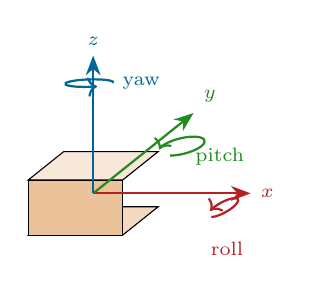
\begin{tikzpicture}[font=\scriptsize, x={(1cm,0cm)}, y={(0.5cm,0.4cm)}, z={(0cm,1cm)}]
					\filldraw[fill=cOrange!25, draw=black] (0,0,0) -- (1.2,0,0) -- (1.2,0.9,0) -- (0,0.9,0) -- cycle;
					\filldraw[fill=cOrange!40, draw=black] (0,0,0) -- (1.2,0,0) -- (1.2,0,0.7) -- (0,0,0.7) -- cycle;
					\filldraw[fill=cOrange!15, draw=black] (0,0,0.7) -- (1.2,0,0.7) -- (1.2,0.9,0.7) -- (0,0.9,0.7) -- cycle;
					\draw[flowarrow, cRed] (0.6,0.45,0.35) -- (2.6,0.45,0.35) node[right] {$x$};
					\draw[flowarrow, cGreen] (0.6,0.45,0.35) -- (0.6,3.0,0.35) node[above right] {$y$};
					\draw[flowarrow, cAccent] (0.6,0.45,0.35) -- (0.6,0.45,2.1) node[above] {$z$};
					\draw[->, cRed, thick] (2.1,0.45,0.05) arc (-90:200:0.12 and 0.3);
					\node[cRed] at (2.3,0.45,-0.35) {roll};
					\draw[->, cAccent, thick] (0.85,0.45,1.75) arc (0:300:0.3 and 0.12);
					\node[cAccent, right] at (0.85,0.45,1.75) {yaw};
					\draw[->, cGreen, thick] (0.6,2.4,0.05) arc (-90:200:0.25 and 0.3);
					\node[cGreen, right] at (0.75,2.5,0.0) {pitch};
				\end{tikzpicture}

				\footnotesize 3 translations + 3 rotations = 6 DOF
			\end{column}
		\end{columns}
	\end{frame}

	\begin{frame}{Mobility (Gr\"ubler--Kutzbach) Criterion}
		\begin{block}{Mobility $M$ = number of independent inputs needed}
			\[
			\textbf{Spatial:}\quad M = 6(n - 1 - j) + \sum_{i=1}^{j} f_i
			\qquad\qquad
			\textbf{Planar:}\quad M = 3(n - 1) - 2j_1 - j_2
			\]
			$n$ = links (\emph{including} the fixed base), $j$ = joints, $f_i$ = DOF of joint $i$,
			$j_1$ = 1-DOF joints, $j_2$ = 2-DOF joints.
		\end{block}
		\begin{columns}[T]
			\begin{column}{0.5\textwidth}
				\begin{itemize}\small
					\item $M > 0$ --- a \textbf{mechanism} with $M$ inputs.
					\item $M = 0$ --- a rigid \textbf{structure}.
					\item $M < 0$ --- over-constrained (pre-loaded) structure.
					\item \textbf{Synthesis}: choose links \& joints so that $M$ equals the number of motors we want.
				\end{itemize}
			\end{column}
			\begin{column}{0.5\textwidth}
				\centering
				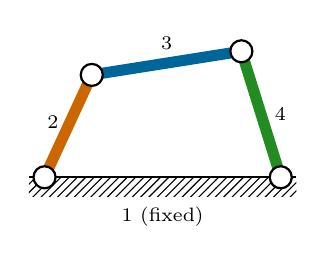
\begin{tikzpicture}[font=\scriptsize]
					% planar four-bar
					\fill[ground] (-0.2,-0.25) rectangle (3.2,0);
					\draw[thick] (-0.2,0) -- (3.2,0);
					\draw[link] (0,0) -- (0.6,1.3);
					\draw[link, cAccent] (0.6,1.3) -- (2.5,1.6);
					\draw[link, cGreen] (2.5,1.6) -- (3.0,0);
					\foreach \p in {(0,0),(0.6,1.3),(2.5,1.6),(3.0,0)} \node[joint] at \p {};
					\node[left] at (0.3,0.7) {2};
					\node[above] at (1.55,1.5) {3};
					\node[right] at (2.8,0.8) {4};
					\node[below] at (1.5,-0.25) {1 (fixed)};
				\end{tikzpicture}

				\footnotesize Four-bar: $n = 4$, $j_1 = 4$\\
				$M = 3(4-1) - 2(4) = \boxed{1}$ --- one motor drives it.
			\end{column}
		\end{columns}
	\end{frame}

	\begin{frame}{Mobility: Worked Examples}
		\renewcommand{\arraystretch}{1.35}
		\centering
		\small
		\begin{tabular}{@{}>{\raggedright}p{3.8cm}cccp{4.4cm}@{}}
			\toprule
			\textbf{Chain} & $\bm{n}$ & \textbf{Joints} & $\bm{M}$ & \textbf{Working} \\
			\midrule
			Planar triangle (3 bars)   & 3 & 3 R & 0 & $3(2) - 2(3) = 0$ \; structure \\
			Planar four-bar            & 4 & 4 R & 1 & $3(3) - 2(4) = 1$ \\
			Planar five-bar            & 5 & 5 R & 2 & $3(4) - 2(5) = 2$ \; 2 motors \\
			Planar 3R open arm         & 4 & 3 R & 3 & $3(3) - 2(3) = 3$ \\
			Spatial 6R robot arm       & 7 & 6 R & 6 & $6(7-1-6) + 6 = 6$ \\
			Spatial 7R (redundant) arm & 8 & 7 R & 7 & $6(8-1-7) + 7 = 7$ \\
			\bottomrule
		\end{tabular}
		\vspace{0.3cm}
		\begin{block}{Serial vs.\ parallel robots}
			\small \textbf{Serial} (open chain): one joint after another --- large workspace, errors add up. \textbf{Parallel} (closed chain, e.g.\ Stewart platform, delta robot): several legs share the load --- stiff, fast, but small workspace.
		\end{block}
	\end{frame}

	% =================================================================
	\section{Elements of Robot Anatomy}
	% =================================================================
	\begin{frame}{Robot Anatomy: Base, Arm, Wrist, End-Effector}
		\begin{columns}[T]
			\begin{column}{0.5\textwidth}
				\centering
				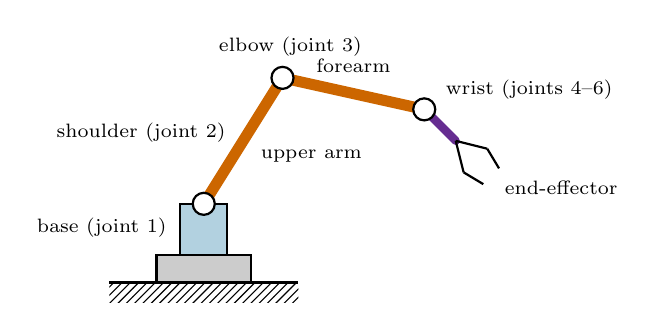
\begin{tikzpicture}[font=\scriptsize]
					\fill[ground] (-1.2,-0.25) rectangle (1.2,0);
					\draw[thick] (-1.2,0) -- (1.2,0);
					\filldraw[fill=gray!40, thick] (-0.6,0) rectangle (0.6,0.35);
					\filldraw[fill=cAccent!30, thick] (-0.3,0.35) rectangle (0.3,1.0);
					\draw[link] (0,1.0) -- (1.0,2.6);
					\draw[link] (1.0,2.6) -- (2.8,2.2);
					\draw[link, line width=3pt, cPurple] (2.8,2.2) -- (3.2,1.8);
					\foreach \p in {(0,1.0),(1.0,2.6),(2.8,2.2)} \node[joint] at \p {};
					\draw[thick] (3.2,1.8) -- (3.3,1.4) (3.2,1.8) -- (3.6,1.7);
					\draw[thick] (3.3,1.4) -- (3.55,1.25) (3.6,1.7) -- (3.75,1.45);
					\node[left] at (-0.35,0.7) {base (joint 1)};
					\node[left] at (0.4,1.9) {shoulder (joint 2)};
					\node[above] at (1.1,2.75) {elbow (joint 3)};
					\node[right] at (2.95,2.45) {wrist (joints 4--6)};
					\node[right] at (3.7,1.2) {end-effector};
					\node at (1.9,2.75) {forearm};
					\node[right] at (0.6,1.6) {upper arm};
				\end{tikzpicture}
			\end{column}
			\begin{column}{0.5\textwidth}
				\begin{itemize}\small
					\item \textbf{Base} --- fixed to the floor, ceiling or a moving track.
					\item \textbf{Arm (body + arm)} --- first 3 joints; \textbf{position} the wrist in space.
					\item \textbf{Wrist} --- last 2--3 joints (roll, pitch, yaw); \textbf{orient} the tool.
					\item \textbf{End-effector} --- gripper or tool mounted on the wrist flange.
					\item \textbf{Tool centre point (TCP)} --- the point the controller moves and programs.
				\end{itemize}
			\end{column}
		\end{columns}
	\end{frame}

	\begin{frame}{Types of Robot Joints}
		\renewcommand{\arraystretch}{1.1}
		\centering
		\footnotesize
		\begin{tabular}{@{}clp{4.4cm}p{4.2cm}@{}}
			\toprule
			\textbf{Symbol} & \textbf{Joint} & \textbf{Relative motion} & \textbf{Axes of input / output links} \\
			\midrule
			\textbf{L} & Linear      & sliding, links \emph{parallel}         & same axis \\
			\textbf{O} & Orthogonal  & sliding, output link \emph{perpendicular} & at right angles \\
			\textbf{R} & Rotational  & rotation, axis \emph{perpendicular} to both links & e.g.\ elbow \\
			\textbf{T} & Twisting    & rotation, axis \emph{parallel} to both links & e.g.\ wrist roll \\
			\textbf{V} & Revolving   & rotation, input link parallel, output perpendicular to axis & e.g.\ base swivel \\
			\bottomrule
		\end{tabular}
		\vspace{0.15cm}
		\begin{block}{Notation}
			\small A robot is described by its arm joints followed by its wrist joints, e.g.\ \textbf{TRR:RT} = articulated arm with a two-joint wrist. L and O are \textbf{prismatic}; R, T and V are \textbf{revolute}.
		\end{block}
	\end{frame}

	\begin{frame}{The Five Common Robot Configurations}
		\centering
		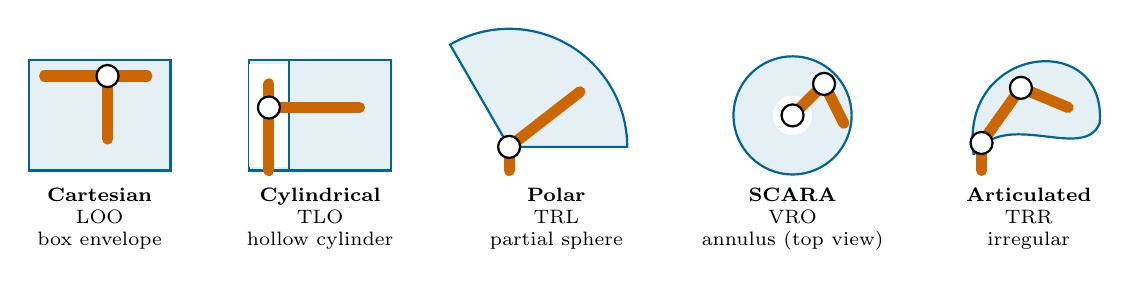
\begin{tikzpicture}[font=\scriptsize]
			% ---- Cartesian ----
			\begin{scope}[shift={(0,0)}]
				\draw[thick, cAccent, fill=cAccent!10] (0,0) rectangle (1.8,1.4);
				\draw[link] (0.2,1.2) -- (1.5,1.2);
				\draw[link] (1.0,1.2) -- (1.0,0.4);
				\node[joint] at (1.0,1.2) {};
				\node[below, align=center] at (0.9,-0.1) {\textbf{Cartesian}\\ LOO\\ box envelope};
			\end{scope}
			% ---- Cylindrical ----
			\begin{scope}[shift={(2.8,0)}]
				\draw[thick, cAccent, fill=cAccent!10] (0,0) rectangle (1.8,1.4);
				\fill[white] (0,0.05) rectangle (0.5,1.35);
				\draw[thick, cAccent] (0.5,0) -- (0.5,1.4);
				\draw[link] (0.25,0) -- (0.25,1.1);
				\draw[link] (0.25,0.8) -- (1.4,0.8);
				\node[joint] at (0.25,0.8) {};
				\node[below, align=center] at (0.9,-0.1) {\textbf{Cylindrical}\\ TLO\\ hollow cylinder};
			\end{scope}
			% ---- Polar ----
			\begin{scope}[shift={(5.8,0)}]
				\filldraw[thick, cAccent, fill=cAccent!10] (0.3,0.3) -- (1.8,0.3) arc (0:120:1.5) -- cycle;
				\draw[link] (0.3,0) -- (0.3,0.3);
				\draw[link] (0.3,0.3) -- (1.2,1.0);
				\node[joint] at (0.3,0.3) {};
				\node[below, align=center] at (0.9,-0.1) {\textbf{Polar}\\ TRL\\ partial sphere};
			\end{scope}
			% ---- SCARA (top view) ----
			\begin{scope}[shift={(8.8,0)}]
				\filldraw[thick, cAccent, fill=cAccent!10] (0.9,0.7) circle (0.75);
				\fill[white] (0.9,0.7) circle (0.25);
				\draw[link] (0.9,0.7) -- (1.3,1.1);
				\draw[link] (1.3,1.1) -- (1.55,0.6);
				\node[joint] at (0.9,0.7) {};
				\node[joint] at (1.3,1.1) {};
				\node[below, align=center] at (0.9,-0.1) {\textbf{SCARA}\\ VRO\\ annulus (top view)};
			\end{scope}
			% ---- Articulated ----
			\begin{scope}[shift={(11.8,0)}]
				\filldraw[thick, cAccent, fill=cAccent!10] (0.2,0.2) .. controls (0.0,1.6) and (1.9,1.8) .. (1.8,0.6) .. controls (1.6,0.1) and (0.6,0.8) .. (0.2,0.2);
				\draw[link] (0.3,0) -- (0.3,0.35);
				\draw[link] (0.3,0.35) -- (0.8,1.05);
				\draw[link] (0.8,1.05) -- (1.4,0.8);
				\node[joint] at (0.3,0.35) {};
				\node[joint] at (0.8,1.05) {};
				\node[below, align=center] at (0.9,-0.1) {\textbf{Articulated}\\ TRR\\ irregular};
			\end{scope}
		\end{tikzpicture}
		\vspace{0.2cm}
		\begin{itemize}\small
			\item \textbf{Work envelope} (work volume) --- all points the wrist can reach; its shape follows from the joint types.
			\item \textbf{Articulated} (jointed-arm) is the most common; \textbf{SCARA} is the fastest for assembly; \textbf{Cartesian} (gantry) is the most accurate \& easiest to program.
		\end{itemize}
	\end{frame}

	\begin{frame}{Comparing Robot Configurations}
		\renewcommand{\arraystretch}{1.25}
		\centering
		\small
		\begin{tabular}{@{}>{\raggedright}p{2.4cm}>{\raggedright}p{1.4cm}>{\raggedright}p{4.0cm}>{\raggedright\arraybackslash}p{4.6cm}@{}}
			\toprule
			\textbf{Configuration} & \textbf{Joints} & \textbf{Advantages} & \textbf{Typical applications} \\
			\midrule
			Cartesian   & LOO & rigid, accurate, simple control   & gantry loading, 3-D printing, palletising \\
			Cylindrical & TLO & simple, large vertical reach      & machine loading, assembly \\
			Polar       & TRL & long horizontal reach             & spot welding, die casting (Unimate) \\
			SCARA       & VRO & very fast, stiff vertically       & electronic assembly, pick-and-place \\
			Articulated & TRR & dexterous, compact footprint      & arc welding, painting, general handling \\
			\bottomrule
		\end{tabular}
		\vspace{0.3cm}
		\begin{block}{Wrist motions}
			\small \textbf{Roll} (twist about the arm axis, T), \textbf{pitch} (up--down, R) and \textbf{yaw} (left--right, R). A 3-DOF arm + 3-DOF wrist = full 6-DOF robot.
		\end{block}
	\end{frame}

	\begin{frame}{Robot Specifications and Precision}
		\begin{columns}[T]
			\begin{column}{0.5\textwidth}
				\begin{block}{Key specifications}
					\begin{itemize}\small
						\item \textbf{Payload} --- mass it can carry at full speed (kg).
						\item \textbf{Reach} --- maximum distance from base to wrist.
						\item \textbf{Speed} --- tool speed (m/s) or cycle time.
						\item \textbf{Spatial resolution} --- smallest move it can make.
						\item \textbf{Accuracy} --- how close it reaches a \emph{commanded} point.
						\item \textbf{Repeatability} --- how close it returns to a \emph{taught} point ($\pm3\sigma$).
					\end{itemize}
				\end{block}
			\end{column}
			\begin{column}{0.5\textwidth}
				\textbf{Example:} a sliding joint has a range of 1.0 m and its position is stored as an \textbf{8-bit} number. Mechanical errors have $\sigma = 0.5$ mm.
				\small
				\begin{align*}
					\text{CR} &= \frac{1000}{2^8} = \frac{1000}{256} = \boxed{3.9\ \text{mm}}\\
					\text{Accuracy} &= \frac{\text{CR}}{2} + 3\sigma = 1.95 + 1.5 = \boxed{3.45\ \text{mm}}\\
					\text{Repeatability} &= \pm3\sigma = \pm1.5\ \text{mm}
				\end{align*}
				\footnotesize With 12 bits, CR $= 1000/4096 = 0.24$ mm --- more bits, finer control.
			\end{column}
		\end{columns}
	\end{frame}

	\begin{frame}{Forward Kinematics of a Two-Link Arm}
		\begin{columns}[T]
			\begin{column}{0.5\textwidth}
				\begin{block}{Forward kinematics}
					\small Given the \textbf{joint angles}, find the \textbf{position} of the gripper.
					\[
					\begin{aligned}
						x &= L_1\cos\theta_1 + L_2\cos(\theta_1+\theta_2)\\
						y &= L_1\sin\theta_1 + L_2\sin(\theta_1+\theta_2)
					\end{aligned}
					\]
				\end{block}
				\begin{block}{Inverse kinematics}
					\small Given the \textbf{position}, find the \textbf{angles} --- what the controller must solve to move in straight lines:
					\[
					\cos\theta_2 = \frac{x^2 + y^2 - L_1^2 - L_2^2}{2L_1L_2}
					\]
				\end{block}
			\end{column}
			\begin{column}{0.5\textwidth}
				\centering
				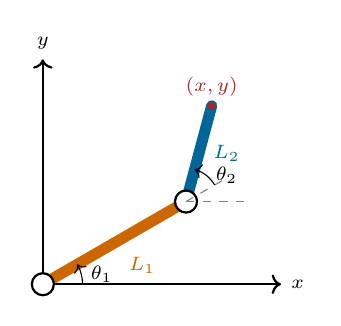
\begin{tikzpicture}[font=\scriptsize, scale=4.2]
					\draw[->, thick] (0,0) -- (0.72,0) node[right] {$x$};
					\draw[->, thick] (0,0) -- (0,0.68) node[above] {$y$};
					\coordinate (O) at (0,0);
					\coordinate (A) at ({0.5*cos(30)},{0.5*sin(30)});
					\coordinate (B) at ({0.5*cos(30)+0.3*cos(75)},{0.5*sin(30)+0.3*sin(75)});
					\draw[link] (O) -- (A) node[midway, below right] {$L_1$};
					\draw[link, cAccent] (A) -- (B) node[midway, right] {$L_2$};
					\node[joint] at (O) {};
					\node[joint] at (A) {};
					\fill[cRed] (B) circle (0.012) node[above] {$(x, y)$};
					\draw[dashed, gray] (A) -- ++(0.2,0);
					\draw[->] (0.12,0) arc (0:30:0.12) node[midway, right] {$\theta_1$};
					\draw[dashed, gray] (A) -- ++({0.15*cos(30)},{0.15*sin(30)});
					\draw[->] ($(A)+({0.1*cos(30)},{0.1*sin(30)})$) arc (30:75:0.1) node[midway, right] {$\theta_2$};
				\end{tikzpicture}

				\footnotesize $L_1 = 0.5$ m, $L_2 = 0.3$ m, $\theta_1 = 30^\circ$, $\theta_2 = 45^\circ$
			\end{column}
		\end{columns}
	\end{frame}

	\begin{frame}[fragile, plain]{}

		\vspace*{0.05cm}

		\begin{columns}[T,onlytextwidth]

			% =========================================================
			% LEFT COLUMN -- PSEUDOCODE
			% =========================================================

			\begin{column}{0.25\textwidth}

				\begin{block}{Pseudocode}
					\scriptsize
					\begin{enumerate}
						\item START
						\item Set $L_1 = 0.5$, $L_2 = 0.3$
						\item READ \texttt{th1}, \texttt{th2} (degrees)
						\item Convert to radians
						\item \texttt{x = L1 cos th1 + L2 cos(th1+th2)}
						\item \texttt{y = L1 sin th1 + L2 sin(th1+th2)}
						\item PRINT \texttt{x}, \texttt{y}
						\item STOP
					\end{enumerate}
				\end{block}

			\end{column}


			% =========================================================
			% MIDDLE COLUMN -- C PROGRAM
			% =========================================================
			\hspace*{0.3cm}
			\begin{column}{0.47\textwidth}

				\begin{block}{C Program (forward kinematics)}

\begin{lstlisting}[style=cstyle,numbers=none,basicstyle=\ttfamily\scriptsize]
#include <stdio.h>
#include <math.h>

#define PI 3.14159265

int main(void)
{
	float L1 = 0.5, L2 = 0.3;  /* metres */
	float t1, t2, x, y;

	printf("th1 th2 (deg): ");
	scanf("%f %f", &t1, &t2);

	t1 = t1 * PI / 180.0;      /* to rad */
	t2 = t2 * PI / 180.0;

	x = L1*cos(t1) + L2*cos(t1 + t2);
	y = L1*sin(t1) + L2*sin(t1 + t2);

	printf("x = %.3f m, y = %.3f m\n", x, y);
	return 0;
}
\end{lstlisting}

				\end{block}

			\end{column}


			% =========================================================
			% RIGHT COLUMN -- NOTES
			% =========================================================

			\begin{column}{0.25\textwidth}

				\begin{tikzpicture}[remember picture,overlay]
					\node[
					anchor=north east,
					draw,
					rounded corners=2pt,
					fill=white,
					text width=3.5cm,
					align=left,
					inner sep=6pt
					] at ([xshift=-2mm,yshift=-6mm]current page.north east)
					{
						\textbf{Program Output}\\[3pt]
						\ttfamily\scriptsize
						th1 th2 (deg): 30 45\\
						x = 0.511 m, y = 0.540 m
					};
				\end{tikzpicture}

			\end{column}

		\end{columns}

		\begin{tikzpicture}[remember picture,overlay]
			\node[
			anchor=south east,
			draw,
			rounded corners=2pt,
			fill=cGrayBg,
			text width=3.5cm,
			align=left,
			inner sep=6pt,
			font=\scriptsize
			] at ([xshift=-2mm,yshift=4mm]current page.south east)
			{
				\textbf{Check by hand:}\\
				$x = 0.433 + 0.078 = 0.511$\\
				$y = 0.250 + 0.290 = 0.540$\\[3pt]
				Compile with \texttt{gcc fk.c -o fk -lm} (\texttt{-lm} links the maths library for \texttt{sin}/\texttt{cos}).
			};
		\end{tikzpicture}

	\end{frame}

	% =================================================================
	\section{Hydraulic, Pneumatic and Electrical Manipulators}
	% =================================================================
	\begin{frame}{Robot Drive Systems}
		\begin{columns}[T]
			\begin{column}{0.32\textwidth}
				\begin{block}{Hydraulic}
					\centering
					\textbf{Pressurised oil}

					\vspace{0.2cm}

					\begin{itemize}\small
						\item Very high payload \& power-to-weight.
						\item Stiff, smooth, holds heavy loads.
						\item Leaks, noise, maintenance.
						\item Early robots (Unimate), heavy handling, forging.
					\end{itemize}
				\end{block}
			\end{column}
			\begin{column}{0.32\textwidth}
				\begin{block}{Pneumatic}
					\centering
					\textbf{Compressed air}

					\vspace{0.2cm}

					\begin{itemize}\small
						\item Cheap, fast, clean, spark-free.
						\item Air compresses $\rightarrow$ poor position control.
						\item Usually moves between \textbf{end stops}.
						\item Pick-and-place, small parts, grippers.
					\end{itemize}
				\end{block}
			\end{column}
			\begin{column}{0.32\textwidth}
				\begin{block}{Electrical}
					\centering
					\textbf{Servo \& stepper motors}

					\vspace{0.2cm}

					\begin{itemize}\small
						\item Accurate, quiet, clean, easy to control.
						\item Needs gearing (harmonic drive, belts).
						\item Lower power-to-weight than hydraulics.
						\item \textbf{Most modern robots}.
					\end{itemize}
				\end{block}
			\end{column}
		\end{columns}
		\vspace{0.3cm}
		\centering\small
		Choice depends on \textbf{payload}, \textbf{accuracy}, \textbf{speed}, \textbf{environment} and \textbf{cost}.
	\end{frame}

	\begin{frame}{Comparing Robot Drive Systems}
		\renewcommand{\arraystretch}{1.1}
		\centering
		\footnotesize
		\begin{tabular}{@{}>{\raggedright}p{3.0cm}>{\raggedright}p{3.2cm}>{\raggedright}p{3.2cm}>{\raggedright\arraybackslash}p{3.2cm}@{}}
			\toprule
			\textbf{Feature} & \textbf{Hydraulic} & \textbf{Pneumatic} & \textbf{Electrical} \\
			\midrule
			Payload            & very high (100s of kg)  & low (a few kg)          & low to high \\
			Positioning        & good (servo valves)     & poor, end-stop only     & excellent \\
			Speed              & medium                  & very high               & high \\
			Explosive areas    & safe (no sparks)        & safe                    & needs special motors \\
			Cleanliness        & oil leaks               & clean                   & clean \\
			Maintenance        & high                    & low                     & low \\
			Typical robot      & heavy / outdoor handling & pick-and-place unit    & welding, assembly, painting \\
			\bottomrule
		\end{tabular}
		\vspace{0.15cm}
		\begin{block}{Key idea}
			\small The same ideas you met for fluid-power and electrical control systems apply here --- a robot is simply several such actuators arranged as a \textbf{kinematic chain}.
		\end{block}
	\end{frame}

	\begin{frame}{Electrical Manipulators: Motors and Transmissions}
		\begin{columns}[T]
			\begin{column}{0.5\textwidth}
				\begin{itemize}\small
					\item \textbf{AC servo motors} (brushless) with encoders --- standard for industrial arms.
					\item \textbf{Stepper motors} --- small, low-cost, open-loop arms and grippers.
					\item \textbf{Harmonic (strain-wave) drive} --- ratios 50--160:1 in one stage, near-zero backlash.
					\item \textbf{Ball screws, belts, rack \& pinion} --- linear axes of gantry robots.
					\item \textbf{Brakes} hold the arm when power fails.
				\end{itemize}
			\end{column}
			\begin{column}{0.5\textwidth}
				\centering
				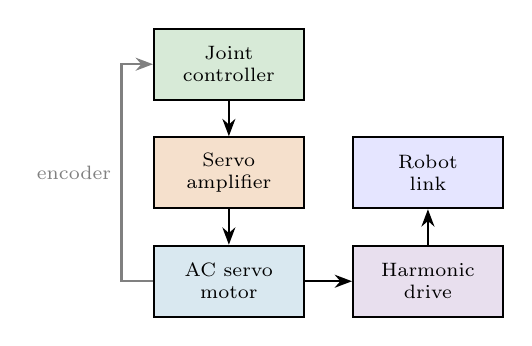
\begin{tikzpicture}[font=\scriptsize, node distance=0.45cm]
					\node[blk, fill=cGreen!18] (c) {Joint\\ controller};
					\node[blk, below=of c, fill=cOrange!20] (a) {Servo\\ amplifier};
					\node[blk, below=of a, fill=cAccent!15] (m) {AC servo\\ motor};
					\node[blk, right=0.6cm of m, fill=cPurple!15] (g) {Harmonic\\ drive};
					\node[blk, above=of g, fill=blue!10] (l) {Robot\\ link};
					\draw[sig] (c) -- (a); \draw[sig] (a) -- (m); \draw[sig] (m) -- (g); \draw[sig] (g) -- (l);
					\draw[sig, gray] (m.west) -- ++(-0.4,0) |- node[pos=0.25, left] {encoder} (c.west);
				\end{tikzpicture}
				\vspace{0.1cm}

				\footnotesize \textbf{Example:} motor 3000 rpm, harmonic drive 100:1 $\Rightarrow$ joint speed $= 30$ rpm $= 180^\circ$/s, with 100$\times$ the motor torque.
			\end{column}
		\end{columns}
	\end{frame}

	% =================================================================
	\section{End-Effectors and their Design}
	% =================================================================
	\begin{frame}{End-Effectors: Grippers and Tools}
		\centering
		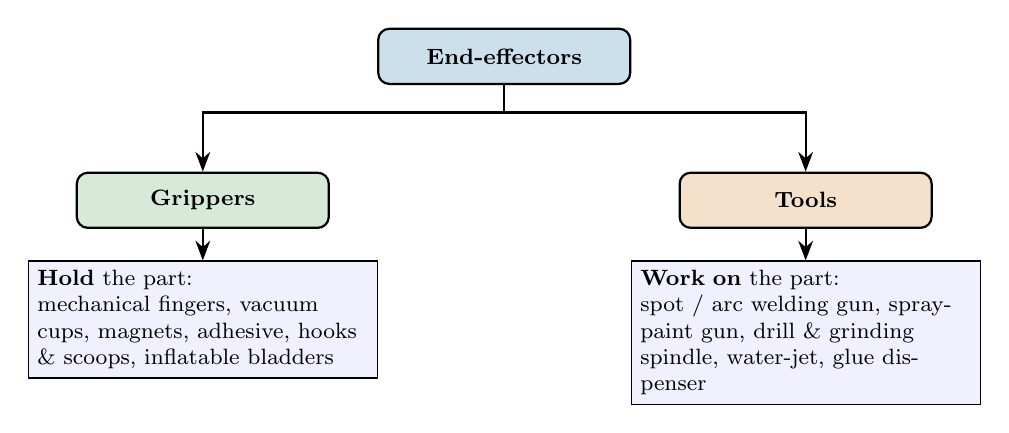
\begin{tikzpicture}[every node/.style={font=\footnotesize},
			hdr/.style={rectangle, draw=black, thick, rounded corners, minimum width=3.2cm, minimum height=0.7cm, align=center, font=\bfseries\footnotesize, fill=cAccent!20},
			grp/.style={rectangle, draw=black, minimum width=3.8cm, align=left, fill=blue!6}]
			\node[hdr] (ee) {End-effectors};
			\node[hdr, below left=1.1cm and 0.6cm of ee, fill=cGreen!18] (gr) {Grippers};
			\node[hdr, below right=1.1cm and 0.6cm of ee, fill=cOrange!20] (tl) {Tools};
			\draw[flowarrow] (ee.south) -- ++(0,-0.35) -| (gr.north);
			\draw[flowarrow] (ee.south) -- ++(0,-0.35) -| (tl.north);
			\node[grp, below=0.4cm of gr, text width=4.2cm] (grc)
			{\textbf{Hold} the part:\\ mechanical fingers, vacuum cups, magnets, adhesive, hooks \& scoops, inflatable bladders};
			\node[grp, below=0.4cm of tl, text width=4.2cm] (tlc)
			{\textbf{Work on} the part:\\ spot / arc welding gun, spray-paint gun, drill \& grinding spindle, water-jet, glue dispenser};
			\draw[flowarrow] (gr) -- (grc);
			\draw[flowarrow] (tl) -- (tlc);
		\end{tikzpicture}
		\vspace{0.2cm}
		\begin{itemize}\small
			\item The end-effector is usually \textbf{custom-designed} for the job --- the robot arm itself is general-purpose.
			\item \textbf{Tool changers} let one robot pick up different end-effectors automatically.
		\end{itemize}
	\end{frame}

	\begin{frame}{Mechanical Grippers}
		\begin{columns}[T]
			\begin{column}{0.5\textwidth}
				\begin{block}{Ways of holding}
					\small \textbf{Friction grip} --- fingers squeeze the part; friction carries the weight.\\
					\textbf{Physical constraint} --- finger shape surrounds the part (form closure).
				\end{block}
				\begin{block}{Actuating mechanisms}
					\begin{itemize}\small
						\item Linkage (toggle) mechanisms.
						\item Rack \& pinion / gear drives.
						\item Cam and screw mechanisms.
						\item Pneumatic cylinder or electric motor as the input.
					\end{itemize}
				\end{block}
			\end{column}
			\begin{column}{0.5\textwidth}
				\centering
				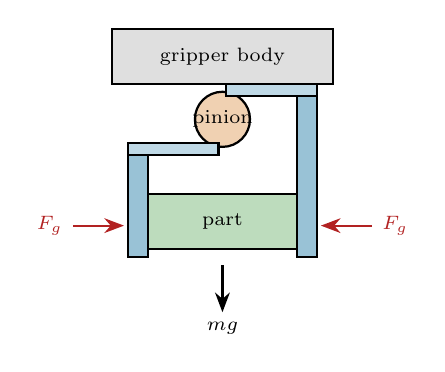
\begin{tikzpicture}[font=\scriptsize]
					% body and rack
					\filldraw[fill=gray!25, thick] (-1.4,1.8) rectangle (1.4,2.5);
					\node at (0,2.15) {gripper body};
					% pinion
					\draw[thick, fill=cOrange!30] (0,1.35) circle (0.35);
					\node at (0,1.35) {pinion};
					% racks
					\filldraw[fill=cAccent!25, thick] (-1.2,0.9) rectangle (-0.05,1.05);
					\filldraw[fill=cAccent!25, thick] (0.05,1.65) rectangle (1.2,1.8);
					% fingers
					\filldraw[fill=cAccent!40, thick] (-1.2,0.9) rectangle (-0.95,-0.4);
					\filldraw[fill=cAccent!40, thick] (0.95,1.65) rectangle (1.2,-0.4);
					% part
					\filldraw[fill=cGreen!30, thick] (-0.95,-0.3) rectangle (0.95,0.4);
					\node at (0,0.05) {part};
					\draw[flowarrow, cRed] (-1.9,0.0) -- (-1.25,0.0) node[pos=0,left] {$F_g$};
					\draw[flowarrow, cRed] (1.9,0.0) -- (1.25,0.0) node[pos=0,right] {$F_g$};
					\draw[flowarrow] (0,-0.5) -- (0,-1.1) node[below] {$mg$};
				\end{tikzpicture}

				\footnotesize Rack-and-pinion parallel gripper: one input moves both fingers equally.
			\end{column}
		\end{columns}
	\end{frame}

	\begin{frame}{Gripper Design: Required Gripping Force}
		\begin{block}{Friction grip}
			The friction force of all fingers must carry the weight \emph{and} the inertia force of the part:
			\[
			\mu\, n_f\, F_g \;\ge\; m\,(g + a)
			\quad\Longrightarrow\quad
			F_g = \frac{m\,(g + a)}{\mu\, n_f}\times\text{SF}
			\]
			$\mu$ = coefficient of friction, $n_f$ = number of contact surfaces (fingers), $a$ = acceleration, SF = safety factor.
		\end{block}
		\begin{columns}[T]
			\begin{column}{0.5\textwidth}
				\textbf{Problem:} a 2 kg part is held between two fingers ($\mu = 0.3$). The robot accelerates it upwards at $10$ m/s$^2$. Use SF $= 2$.
			\end{column}
			\begin{column}{0.5\textwidth}
				\small
				\begin{align*}
					F_g &= \frac{2\,(9.81 + 10)}{0.3\times2} = 66.0\ \text{N}\\
					F_g\ (\text{SF} = 2) &= \boxed{132\ \text{N}}
				\end{align*}
				\footnotesize Rubber finger pads (higher $\mu$) lower the force needed --- and the risk of crushing the part.
			\end{column}
		\end{columns}
	\end{frame}

	\begin{frame}{Vacuum, Magnetic and Other Grippers}
		\begin{columns}[T]
			\begin{column}{0.5\textwidth}
				\begin{block}{Vacuum cups}
					\small Lift force $F = \Delta p\,A$. Ideal for flat, smooth sheets --- glass, sheet metal, cartons.
				\end{block}
				\textbf{Example:} lift a 5 kg steel plate with one cup, vacuum $\Delta p = 60$ kPa, SF $= 2$.
				\small
				\begin{align*}
					A &= \frac{\text{SF}\cdot m g}{\Delta p} = \frac{2\times5\times9.81}{60\,000} = 1.64\times10^{-3}\ \text{m}^2\\
					D &= \sqrt{\tfrac{4A}{\pi}} \approx \boxed{46\ \text{mm}}
				\end{align*}
			\end{column}
			\begin{column}{0.5\textwidth}
				\begin{block}{Magnetic grippers}
					\small Electromagnets or permanent magnets for \textbf{ferrous} parts --- fast pick-up of steel plates, any shape; residual magnetism must be removed.
				\end{block}
				\begin{block}{Others}
					\small Adhesive grippers (fabric, light parts), hooks \& scoops (bags, liquids), inflatable bladders (fragile or irregular parts), soft robotic fingers.
				\end{block}
			\end{column}
		\end{columns}
	\end{frame}

	\begin{frame}{End-Effector Design Considerations}
		\renewcommand{\arraystretch}{1.1}
		\centering
		\footnotesize
		\begin{tabular}{@{}>{\raggedright}p{3.4cm}>{\raggedright\arraybackslash}p{9.2cm}@{}}
			\toprule
			\textbf{Consideration} & \textbf{Question to ask} \\
			\midrule
			Part properties   & mass, size, shape, surface finish, fragility, temperature, magnetic? \\
			Gripping method   & friction or form closure? vacuum or magnet possible? \\
			Force \& weight   & grip force with SF; end-effector mass counts against the robot payload \\
			Tolerances        & how accurately must the part be located? need compliance? \\
			Sensing           & part-present switch, force sensor, vision for location? \\
			Power \& utilities & air, vacuum, electric --- routed through the wrist \\
			Changeover        & quick-change or automatic tool changer for different parts? \\
			\bottomrule
		\end{tabular}
		\vspace{0.15cm}
		\begin{block}{Remote centre compliance (RCC)}
			\small A passive wrist device that lets the part \textbf{tilt and shift slightly} during insertion --- so a peg can enter a hole even when the robot is a little misaligned.
		\end{block}
	\end{frame}

	% =================================================================
	\section{Controllers with Microprocessors or Fluidics}
	% =================================================================
	\begin{frame}{Levels of Robot Control}
		\renewcommand{\arraystretch}{1.1}
		\centering
		\footnotesize
		\begin{tabular}{@{}>{\raggedright}p{3.4cm}>{\raggedright}p{5.6cm}>{\raggedright\arraybackslash}p{3.6cm}@{}}
			\toprule
			\textbf{Type} & \textbf{How it works} & \textbf{Controller} \\
			\midrule
			Limited-sequence (bang-bang) & joints move between \textbf{mechanical stops}; sequence set by a timer or logic & fluidic logic, PLC, cams \\
			Playback, point-to-point     & taught points stored; path between them not controlled & microprocessor \\
			Playback, continuous path    & whole path controlled (straight lines, arcs) by interpolation & microprocessor / DSP \\
			Intelligent                  & uses sensors \& vision to change its actions; makes decisions & multi-processor, PC, AI \\
			\bottomrule
		\end{tabular}
		\vspace{0.15cm}
		\begin{block}{Key idea}
			\small The simplest robots need only \textbf{ON/OFF logic} --- which can be built from \textbf{air} (fluidics). Servo-controlled robots need a \textbf{microprocessor} to calculate and close the loops.
		\end{block}
	\end{frame}

	\begin{frame}{Microprocessor-Based Robot Controller}
		\centering
		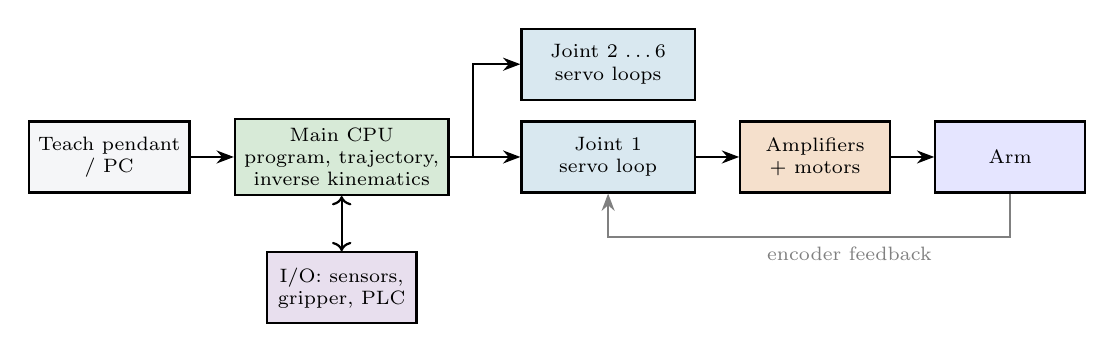
\begin{tikzpicture}[font=\scriptsize, node distance=0.55cm]
			\node[blk, fill=cGrayBg] (tp) {Teach pendant\\ / PC};
			\node[blk, right=of tp, fill=cGreen!18, minimum width=2.4cm] (cpu) {Main CPU\\ program, trajectory,\\ inverse kinematics};
			\node[blk, right=0.9cm of cpu, fill=cAccent!15, minimum width=2.2cm] (j1) {Joint 1\\ servo loop};
			\node[blk, above=0.25cm of j1, fill=cAccent!15, minimum width=2.2cm] (j0) {Joint 2 \dots 6\\ servo loops};
			\node[blk, right=of j1, fill=cOrange!20] (amp) {Amplifiers\\ + motors};
			\node[blk, right=of amp, fill=blue!10] (arm) {Arm};
			\node[blk, below=0.7cm of cpu, fill=cPurple!15] (io) {I/O: sensors,\\ gripper, PLC};
			\draw[sig] (tp) -- (cpu);
			\draw[sig] (cpu) -- (j1);
			\draw[sig] (cpu.east) -- ++(0.3,0) |- (j0.west);
			\draw[sig] (j1) -- (amp);
			\draw[sig] (amp) -- (arm);
			\draw[sig, gray] (arm.south) -- ++(0,-0.55) -| node[pos=0.2, below] {encoder feedback} (j1.south);
			\draw[<->, thick] (cpu) -- (io);
		\end{tikzpicture}
		\vspace{0.25cm}
		\begin{itemize}\small
			\item \textbf{Main processor}: interprets the program, plans the path, solves inverse kinematics every few ms.
			\item \textbf{Joint processors / DSPs}: run a PID position loop for each joint at 1--10 kHz.
			\item \textbf{I/O}: signals to/from grippers, conveyors, machine tools and safety fences (interlocks).
		\end{itemize}
	\end{frame}

	\begin{frame}{How a Robot Controller Runs: The Motion Cycle}
		\vspace*{-0.3cm}
		\begin{block}{The Read---Plan---Solve---Drive cycle}
			Just like the CPU's machine cycle, the robot controller repeats one cycle every
			\textbf{interpolation period} (typically 1--10 ms) while the robot is moving.
		\end{block}
		\begin{columns}[T]
			\begin{column}{0.55\textwidth}
				\begin{enumerate}\small
					\item \textbf{Read} --- next program step and all sensor inputs.
					\item \textbf{Plan} --- next point on the path (straight line / arc) in $x, y, z$.
					\item \textbf{Solve} --- inverse kinematics: joint angles for that point.
					\item \textbf{Drive} --- send the angles to the joint servo loops (PID).
					\item \textbf{Check} --- encoders, limits, collision \& safety signals; then repeat.
				\end{enumerate}
			\end{column}
			\begin{column}{0.45\textwidth}
				\centering
				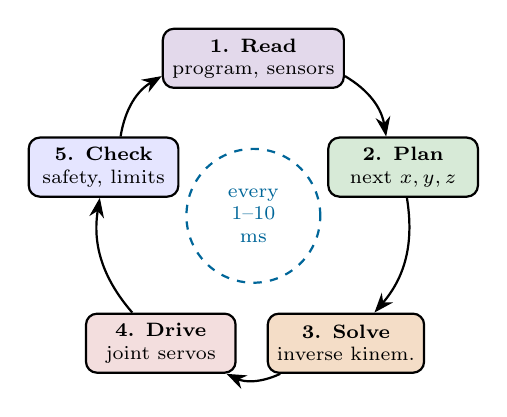
\begin{tikzpicture}[font=\scriptsize,
					stage/.style={rectangle, rounded corners=4pt, draw=black, thick,
						minimum width=1.9cm, minimum height=0.75cm, align=center}]
					\node[circle, draw=cAccent, thick, dashed, minimum size=1.7cm, align=center, text=cAccent]
					(c) at (0,0) {every\\ 1--10\\ ms};
					\node[stage, fill=cPurple!18] (r) at (90:2.0)   {\textbf{1. Read}\\ program, sensors};
					\node[stage, fill=cGreen!18]  (p) at (18:2.0)   {\textbf{2. Plan}\\ next $x, y, z$};
					\node[stage, fill=cOrange!22] (s) at (-54:2.0)  {\textbf{3. Solve}\\ inverse kinem.};
					\node[stage, fill=cRed!15]    (d) at (-126:2.0) {\textbf{4. Drive}\\ joint servos};
					\node[stage, fill=blue!10]    (k) at (162:2.0)  {\textbf{5. Check}\\ safety, limits};
					\draw[flowarrow] (r) to[bend left=25] (p);
					\draw[flowarrow] (p) to[bend left=25] (s);
					\draw[flowarrow] (s) to[bend left=25] (d);
					\draw[flowarrow] (d) to[bend left=25] (k);
					\draw[flowarrow] (k) to[bend left=25] (r);
				\end{tikzpicture}
			\end{column}
		\end{columns}
	\end{frame}

	\begin{frame}{Fluidic Controllers}
		\begin{columns}[T]
			\begin{column}{0.55\textwidth}
				\begin{block}{Fluidics}
					\small Logic built from \textbf{air (or liquid) jets} in channels with \textbf{no moving parts}. A jet sticks to one wall (\textbf{Coanda effect}); a small control jet switches it to the other wall --- a binary 0/1 element.
				\end{block}
				\begin{itemize}\small
					\item Gates: AND, OR, NOT, NOR, flip-flop (memory), timers.
					\item Drive pneumatic cylinders directly --- ideal for \textbf{limited-sequence} pick-and-place robots.
					\item Immune to heat, radiation, magnetic fields, explosive atmospheres.
					\item Slow (ms) and bulky compared with electronics; no arithmetic.
				\end{itemize}
			\end{column}
			\begin{column}{0.45\textwidth}
				\centering
				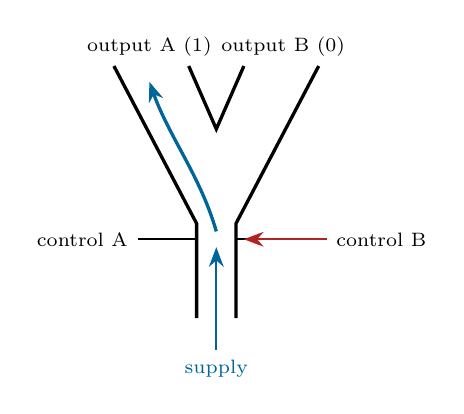
\begin{tikzpicture}[font=\scriptsize]
					% wall-attachment flip-flop
					\draw[very thick] (-0.25,0) -- (-0.25,1.2) -- (-1.3,3.2);
					\draw[very thick] (0.25,0) -- (0.25,1.2) -- (1.3,3.2);
					\draw[very thick] (-0.35,3.2) -- (0,2.4) -- (0.35,3.2);
					\draw[flowarrow, cAccent] (0,-0.4) -- (0,0.9) node[pos=0, below] {supply};
					\draw[flowarrow, cAccent, very thick] (0,1.1) .. controls (-0.2,1.8) and (-0.6,2.3) .. (-0.85,3.0);
					\node[above] at (-0.85,3.2) {output A (1)};
					\node[above] at (0.85,3.2) {output B (0)};
					\draw[thick] (-0.25,1.0) -- (-1.0,1.0);
					\draw[thick] (0.25,1.0) -- (1.0,1.0);
					\draw[flowarrow, cRed] (1.4,1.0) -- (0.35,1.0);
					\node[right] at (1.4,1.0) {control B};
					\node[left] at (-1.0,1.0) {control A};
				\end{tikzpicture}

				\footnotesize Wall-attachment flip-flop: a pulse at \emph{control B} pushes the jet to output B, where it stays.
			\end{column}
		\end{columns}
	\end{frame}

	\begin{frame}{Microprocessor vs.\ Fluidic Control}
		\renewcommand{\arraystretch}{1.3}
		\centering
		\small
		\begin{tabular}{@{}>{\raggedright}p{3.2cm}>{\raggedright}p{4.6cm}>{\raggedright\arraybackslash}p{4.6cm}@{}}
			\toprule
			\textbf{Feature} & \textbf{Microprocessor} & \textbf{Fluidic} \\
			\midrule
			Signal         & electrical (bits in memory)     & air-jet pressure (0/1) \\
			Speed          & $\mu$s per operation            & ms per operation \\
			Functions      & arithmetic, kinematics, PID, vision & ON/OFF logic, sequencing only \\
			Programming    & software --- easy to change     & re-plumb the circuit \\
			Environment    & needs protection from heat, EMI, sparks & works in explosive, hot, radioactive areas \\
			Typical robot  & servo, continuous-path, intelligent & limited-sequence, pneumatic \\
			\bottomrule
		\end{tabular}
		\vspace{0.3cm}
		\begin{block}{Key idea}
			\small Today microprocessors dominate; fluidics survive where \textbf{electricity is dangerous} --- e.g.\ paint booths and cargo areas with flammable vapour.
		\end{block}
	\end{frame}

	\begin{frame}[fragile]{Programming the Robot}
		\begin{columns}[T]
			\begin{column}{0.5\textwidth}
				\begin{block}{Methods}
					\begin{itemize}\small
						\item \textbf{Lead-through (manual)} --- operator physically guides the arm; motion recorded (painting).
						\item \textbf{Teach pendant} --- jog the robot with buttons, store points.
						\item \textbf{Robot language} --- text program (VAL, KRL, RAPID).
						\item \textbf{Off-line} --- simulate in software, download the program.
					\end{itemize}
				\end{block}
			\end{column}
			\begin{column}{0.5\textwidth}
				\textbf{A pick-and-place program (VAL style)}
\begin{lstlisting}[style=valstyle]
PROGRAM PICKPLACE
  SPEED 50            ; % of maximum
  OPENI               ; open gripper
  APPRO PICK, 50      ; 50 mm above
  MOVES PICK          ; straight down
  CLOSEI              ; grip the part
  DEPARTS 50          ; lift straight up
  APPRO PLACE, 50
  MOVES PLACE
  OPENI               ; release
  DEPARTS 50
END
\end{lstlisting}
			\end{column}
		\end{columns}
	\end{frame}

	% =================================================================
	\section{Robot Sensors}
	% =================================================================
	\begin{frame}{Classification of Robot Sensors}
		\centering
		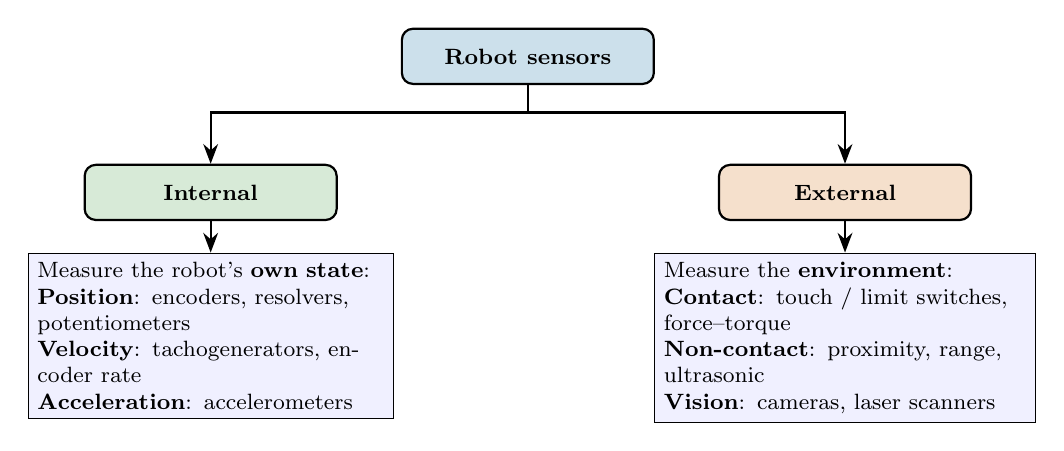
\begin{tikzpicture}[every node/.style={font=\footnotesize},
			hdr/.style={rectangle, draw=black, thick, rounded corners, minimum width=3.2cm, minimum height=0.7cm, align=center, font=\bfseries\footnotesize, fill=cAccent!20},
			grp/.style={rectangle, draw=black, minimum width=3.8cm, align=left, fill=blue!6}]
			\node[hdr] (s) {Robot sensors};
			\node[hdr, below left=1.0cm and 0.8cm of s, fill=cGreen!18] (in) {Internal};
			\node[hdr, below right=1.0cm and 0.8cm of s, fill=cOrange!20] (ex) {External};
			\draw[flowarrow] (s.south) -- ++(0,-0.35) -| (in.north);
			\draw[flowarrow] (s.south) -- ++(0,-0.35) -| (ex.north);
			\node[grp, below=0.4cm of in, text width=4.4cm] (inc)
			{Measure the robot's \textbf{own state}:\\
				\textbf{Position}: encoders, resolvers, potentiometers\\
				\textbf{Velocity}: tachogenerators, encoder rate\\
				\textbf{Acceleration}: accelerometers};
			\node[grp, below=0.4cm of ex, text width=4.6cm] (exc)
			{Measure the \textbf{environment}:\\
				\textbf{Contact}: touch / limit switches, force--torque\\
				\textbf{Non-contact}: proximity, range, ultrasonic\\
				\textbf{Vision}: cameras, laser scanners};
			\draw[flowarrow] (in) -- (inc);
			\draw[flowarrow] (ex) -- (exc);
		\end{tikzpicture}
		\vspace{0.2cm}

		\small Internal sensors close the \textbf{servo loops}; external sensors let the robot \textbf{react} to the world.
	\end{frame}

	\begin{frame}{Internal Sensors: Encoders}
		\begin{columns}[T]
			\begin{column}{0.5\textwidth}
				\begin{block}{Incremental encoder}
					\small A disc with $N$ slots gives $N$ pulses/rev; two channels (A, B) $90^\circ$ apart give direction and $4N$ counts/rev (quadrature). Needs a \textbf{homing} run at start-up.
				\end{block}
				\begin{block}{Absolute encoder}
					\small Each position has a unique binary (Gray) code on $n$ tracks: $2^n$ positions/rev. Knows its position at power-on.
				\end{block}
			\end{column}
			\begin{column}{0.5\textwidth}
				\centering
				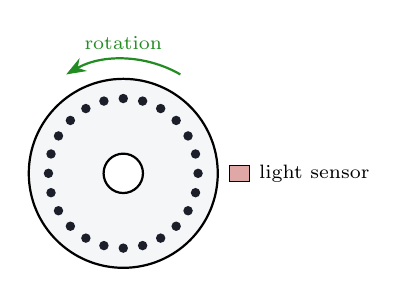
\begin{tikzpicture}[font=\scriptsize]
					\draw[thick, fill=cGrayBg] (0,0) circle (1.2);
					\foreach \a in {0,15,...,345} \fill[cBox] (\a:0.95) circle (0.06);
					\draw[thick, fill=white] (0,0) circle (0.25);
					\draw[flowarrow, cGreen] (60:1.45) arc (60:120:1.45);
					\node[cGreen] at (90:1.65) {rotation};
					\filldraw[fill=cRed!40] (1.35,-0.1) rectangle (1.6,0.1);
					\node[right] at (1.6,0) {light sensor};
				\end{tikzpicture}
				\vspace{0.2cm}

				\small
				\textbf{Examples:}\\
				12-bit absolute: $360^\circ/4096 = \boxed{0.088^\circ}$\\
				1000-line incremental, $\times4$: $360^\circ/4000 = \boxed{0.09^\circ}$
			\end{column}
		\end{columns}
		\vspace{0.1cm}
		\footnotesize\centering Through a 100:1 gear the joint resolution becomes 100 times finer.
	\end{frame}

	\begin{frame}{External Sensors: Touch, Force, Proximity and Range}
		\renewcommand{\arraystretch}{1.1}
		\centering
		\footnotesize
		\begin{tabular}{@{}>{\raggedright}p{2.8cm}>{\raggedright}p{5.0cm}>{\raggedright\arraybackslash}p{4.6cm}@{}}
			\toprule
			\textbf{Sensor} & \textbf{Principle} & \textbf{Robot use} \\
			\midrule
			Touch / limit switch & contact closes a switch               & part present in gripper \\
			Tactile array        & grid of pressure cells in finger pads  & shape \& slip detection \\
			Force--torque (wrist) & strain gauges measure 6 components    & assembly, polishing, collision \\
			Inductive proximity  & eddy currents from metal (a few mm)   & detect metal parts \\
			Capacitive proximity & capacitance change, any material     & level, non-metal parts \\
			Ultrasonic / optical & time of flight or reflected light     & distance, obstacle avoidance \\
			\bottomrule
		\end{tabular}
		\vspace{0.15cm}
		\begin{block}{Range by time of flight}
			\small $d = \dfrac{v\,t}{2}$ \quad e.g.\ ultrasonic echo after $t = 2$ ms, $v = 343$ m/s $\Rightarrow d = \dfrac{343\times0.002}{2} = \boxed{0.343\ \text{m}}$
		\end{block}
	\end{frame}

	\begin{frame}{Machine Vision}
		\begin{block}{Machine vision}
			A camera and computer that let the robot \textbf{see}: find a part's position and orientation, check its quality, or read codes.
		\end{block}
		\centering
		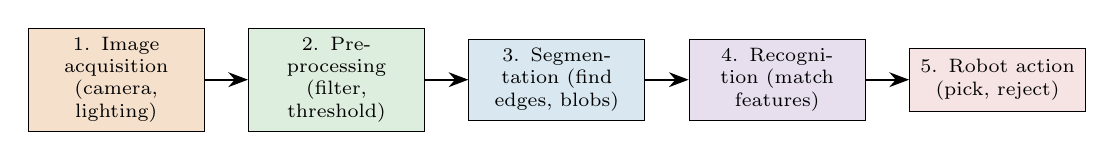
\begin{tikzpicture}[every node/.style={font=\scriptsize}, node distance=0.55cm]
			\node[process, minimum width=2.0cm, text width=2.0cm, fill=cOrange!20] (p1){1. Image acquisition (camera, lighting)};
			\node[process, right=of p1, minimum width=2.0cm, text width=2.0cm, fill=cGreen!15] (p2){2. Pre-processing (filter, threshold)};
			\node[process, right=of p2, minimum width=2.0cm, text width=2.0cm, fill=cAccent!15] (p3){3. Segmentation (find edges, blobs)};
			\node[process, right=of p3, minimum width=2.0cm, text width=2.0cm, fill=cPurple!15] (p4){4. Recognition (match features)};
			\node[process, right=of p4, minimum width=2.0cm, text width=2.0cm, fill=cRed!12] (p5){5. Robot action (pick, reject)};
			\draw[flowarrow](p1)--(p2); \draw[flowarrow](p2)--(p3); \draw[flowarrow](p3)--(p4); \draw[flowarrow](p4)--(p5);
		\end{tikzpicture}
		\vspace{0.3cm}
		\begin{itemize}\small
			\item \textbf{Bin picking} --- find randomly placed parts; \textbf{seam tracking} --- follow a weld joint.
			\item \textbf{Inspection} --- measure dimensions, detect defects at production speed.
			\item Good \textbf{lighting} is half the job --- back-lighting gives sharp silhouettes.
		\end{itemize}
	\end{frame}

	% =================================================================
	\section{Applications of Industrial Robots}
	% =================================================================
	\begin{frame}{Characteristics of Jobs Suitable for Robots}
		\begin{columns}[T]
			\begin{column}{0.5\textwidth}
				\begin{block}{A job is a good robot candidate when it is}
					\begin{itemize}\small
						\item \textbf{Hazardous} or uncomfortable for people (heat, fumes, paint, radiation).
						\item \textbf{Repetitive} with a steady work cycle.
						\item Handling parts that are \textbf{heavy} or awkward.
						\item Run over \textbf{multiple shifts}.
						\item Needs \textbf{consistent quality} (welds, paint thickness).
						\item Parts arrive at a \textbf{known position} and orientation.
					\end{itemize}
				\end{block}
			\end{column}
			\begin{column}{0.5\textwidth}
				\begin{block}{Work-cell layouts}
					\small
					\textbf{Robot-centred} --- robot in the middle serving machines around it.\\[3pt]
					\textbf{In-line} --- robots along a conveyor (car body welding).\\[3pt]
					\textbf{Mobile} --- robot on a track or AGV serving several machines.
				\end{block}
				\centering
				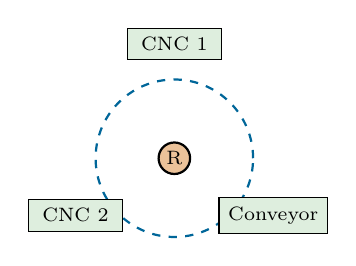
\begin{tikzpicture}[font=\scriptsize]
					\draw[thick, dashed, cAccent] (0,0) circle (1.0);
					\node[joint, minimum size=0.4cm, fill=cOrange!40] at (0,0) {R};
					\foreach \a/\n in {90/CNC 1, 210/CNC 2, 330/Conveyor}
					\node[rectangle, draw, fill=cGreen!15, minimum width=1.2cm] at (\a:1.45) {\n};
				\end{tikzpicture}
			\end{column}
		\end{columns}
	\end{frame}

	\begin{frame}{Applications of Industrial Robots}
		\begin{columns}[T]
			\begin{column}{0.32\textwidth}
				\begin{block}{Material handling}
					\begin{itemize}\small
						\item Pick-and-place, transfer.
						\item Palletising / packing.
						\item \textbf{Machine loading}: CNC, presses, die casting, forging.
					\end{itemize}
				\end{block}
			\end{column}
			\begin{column}{0.32\textwidth}
				\begin{block}{Processing}
					\begin{itemize}\small
						\item \textbf{Spot \& arc welding}.
						\item \textbf{Spray painting}, coating.
						\item Grinding, deburring, polishing, cutting (laser, water-jet).
					\end{itemize}
				\end{block}
			\end{column}
			\begin{column}{0.32\textwidth}
				\begin{block}{Assembly \& inspection}
					\begin{itemize}\small
						\item Inserting, screwing, gluing.
						\item Electronic PCB assembly (SCARA).
						\item Vision / probe inspection.
					\end{itemize}
				\end{block}
			\end{column}
		\end{columns}
		\vspace{0.3cm}
		\begin{block}{Marine and shipbuilding applications}
			\small Welding robots for hull blocks and double-bottom sections; plasma / laser profile cutting of plates; hull-blasting and painting crawlers; underwater ROVs for hull inspection, cleaning and offshore maintenance; tank-cleaning robots.
		\end{block}
	\end{frame}

	\begin{frame}{Application Example: Robotic Arc Welding Cell}
		\begin{columns}[T]
			\begin{column}{0.5\textwidth}
				\centering
				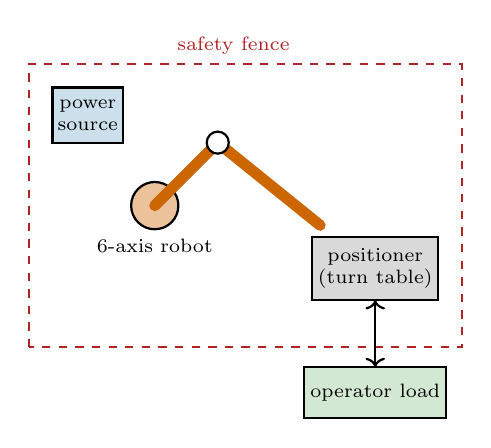
\begin{tikzpicture}[font=\scriptsize]
					% fence
					\draw[thick, dashed, cRed] (-0.2,-0.2) rectangle (5.3,3.4);
					\node[cRed, above] at (2.4,3.4) {safety fence};
					% positioner
					\filldraw[fill=gray!30, thick] (3.4,0.4) rectangle (5.0,1.2);
					\node[align=center] at (4.2,0.8) {positioner\\ (turn table)};
					% robot
					\node[joint, minimum size=0.6cm, fill=cOrange!40] (r) at (1.4,1.6) {};
					\draw[link] (1.4,1.6) -- (2.2,2.4);
					\draw[link] (2.2,2.4) -- (3.5,1.35);
					\node[joint] at (2.2,2.4) {};
					\node[below] at (1.4,1.3) {6-axis robot};
					% power source
					\filldraw[fill=cAccent!20, thick] (0.1,2.4) rectangle (1.0,3.1);
					\node[align=center] at (0.55,2.75) {power\\ source};
					% operator station
					\filldraw[fill=cGreen!20, thick] (3.3,-1.1) rectangle (5.1,-0.45);
					\node[align=center] at (4.2,-0.775) {operator load};
					\draw[<->, thick] (4.2,-0.45) -- (4.2,0.4);
				\end{tikzpicture}
			\end{column}
			\begin{column}{0.5\textwidth}
				\begin{itemize}\small
					\item Robot carries a MIG/MAG welding torch as its end-effector.
					\item \textbf{Positioner} turns the part so welds are made in the flat (down-hand) position.
					\item \textbf{Seam tracking} (arc or laser sensor) corrects for fit-up errors.
					\item Two stations: the operator loads one while the robot welds the other.
					\item Typical gain: arc-on time rises from $\sim$30\,\% (manual) to 80--90\,\%.
				\end{itemize}
			\end{column}
		\end{columns}
	\end{frame}

	% =================================================================
	\section{Economics of Robotics}
	% =================================================================
	\begin{frame}{Costs and Benefits of a Robot Installation}
		\begin{columns}[T]
			\begin{column}{0.5\textwidth}
				\begin{block}{Investment costs}
					\begin{itemize}\small
						\item Robot arm + controller.
						\item End-effectors, fixtures, positioners.
						\item Safety fencing, sensors, conveyors.
						\item Engineering, installation, programming, training.
					\end{itemize}
					\footnotesize The robot itself is often only \textbf{30--50\,\%} of the total project cost.
				\end{block}
			\end{column}
			\begin{column}{0.5\textwidth}
				\begin{block}{Operating costs vs.\ savings}
					\begin{itemize}\small
						\item \textbf{Costs}: maintenance, power, tooling, programming changes.
						\item \textbf{Savings}: direct labour, higher output, less scrap \& rework, lower injury costs, consistent quality.
					\end{itemize}
				\end{block}
				\begin{block}{Justification methods}
					\small Payback period, return on investment (ROI), net present value (NPV).
				\end{block}
			\end{column}
		\end{columns}
	\end{frame}

	\begin{frame}{Payback and ROI: Worked Example}
		\begin{block}{Relations}
			\[
			\text{Payback} = \frac{\text{total investment}}{\text{net annual saving}}
			\qquad
			\text{ROI} = \frac{\text{net annual saving}}{\text{total investment}}\times100\,\%
			\]
		\end{block}
		\begin{columns}[T]
			\begin{column}{0.5\textwidth}
				\textbf{Problem:} a machine-loading robot costs Rs 30 lakh; installation, gripper and fencing add Rs 10 lakh. It replaces one operator on each of two shifts \emph{and} a relief worker for each (4 people, Rs 4 lakh/year each). Robot running costs are Rs 4 lakh/year.
			\end{column}
			\begin{column}{0.5\textwidth}
				\small
				\begin{align*}
					\text{Investment} &= 30 + 10 = 40\ \text{lakh}\\
					\text{Labour saving} &= 4\times4 = 16\ \text{lakh/yr}\\
					\text{Net saving} &= 16 - 4 = 12\ \text{lakh/yr}\\
					\text{Payback} &= 40/12 \approx \boxed{3.3\ \text{years}}\\
					\text{ROI} &= 12/40 = \boxed{30\,\%}
				\end{align*}
			\end{column}
		\end{columns}
		\vspace{0.1cm}
		\footnotesize\centering Most companies accept a robot project if the payback is below 2--3 years; here extra output or quality savings would be needed.
	\end{frame}

	\begin{frame}{Cumulative Cash Flow and Break-Even}
		\begin{columns}[T]
			\begin{column}{0.55\textwidth}
				\centering
				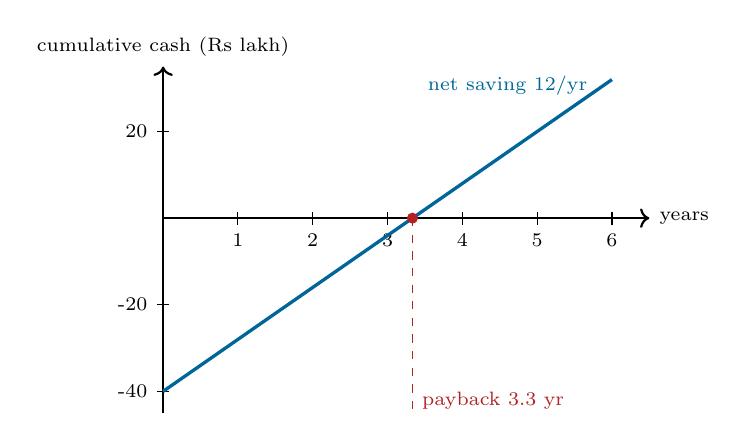
\begin{tikzpicture}[font=\scriptsize, x=0.95cm, y=0.055cm]
					\draw[->, thick] (0,0) -- (6.5,0) node[right] {years};
					\draw[->, thick] (0,-45) -- (0,35) node[above] {cumulative cash (Rs lakh)};
					\foreach \t in {1,...,6} \draw (\t,1.5) -- (\t,-1.5) node[below] {\t};
					\foreach \c in {-40,-20,20} \draw (0.08,\c) -- (-0.08,\c) node[left] {\c};
					\draw[very thick, cAccent] (0,-40) -- (6,32);
					\fill[cRed] (3.333,0) circle (2pt);
					\draw[dashed, cRed] (3.333,0) -- (3.333,-45);
					\node[cRed, below right] at (3.333,-38) {payback 3.3 yr};
					\node[cAccent, above left] at (5.8,26) {net saving 12/yr};
				\end{tikzpicture}
			\end{column}
			\begin{column}{0.45\textwidth}
				\begin{itemize}\small
					\item Start at $-$Rs 40 lakh (investment).
					\item Each year adds Rs 12 lakh of net savings.
					\item The line crosses zero at the \textbf{payback point}.
					\item Over a 6-year life the robot earns Rs 32 lakh more than it cost.
				\end{itemize}
				\vspace{0.2cm}
				\begin{block}{Ways to improve the case}
					\small Run 3 shifts, serve 2 machines with one robot, count quality \& safety savings.
				\end{block}
			\end{column}
		\end{columns}
	\end{frame}

	\begin{frame}{Summary \& What Comes Next}
		\begin{columns}[T]
			\begin{column}{0.5\textwidth}
				\begin{block}{Concept}
					\begin{itemize}\small
						\item Robots: definition, history, system components.
						\item Links, joints, DOF and the mobility criterion.
						\item Robot anatomy, configurations, specifications, kinematics.
						\item Hydraulic, pneumatic and electrical manipulators.
						\item End-effectors and gripper design.
						\item Microprocessor and fluidic controllers; programming.
						\item Sensors, applications and economics.
					\end{itemize}
				\end{block}
			\end{column}
			\begin{column}{0.5\textwidth}
				\begin{block}{Practice makes perfect}
					\begin{itemize}\small
						\item Compute the mobility of mechanisms around you.
						\item Run the kinematics C program for other angles; add inverse kinematics.
						\item Size a gripper for a part of your choice.
					\end{itemize}
				\end{block}
				\begin{block}{Coming up}
					\small Robot kinematics \& dynamics, trajectory planning, and marine / underwater robotics.
				\end{block}
			\end{column}
		\end{columns}
	\end{frame}

	%------------------------------------------------
	\begin{frame}
		\centering
		\Huge Thank You
		\vspace{0.5cm}

		\normalsize Questions?
	\end{frame}

	%------------------------------------------------

\end{document}
